\subsection{SE-10 Consultar lista de asistencia de alumnos inscritos a los ETS}

\begin{figure}[htbp!]
	\begin{center}
		\fbox{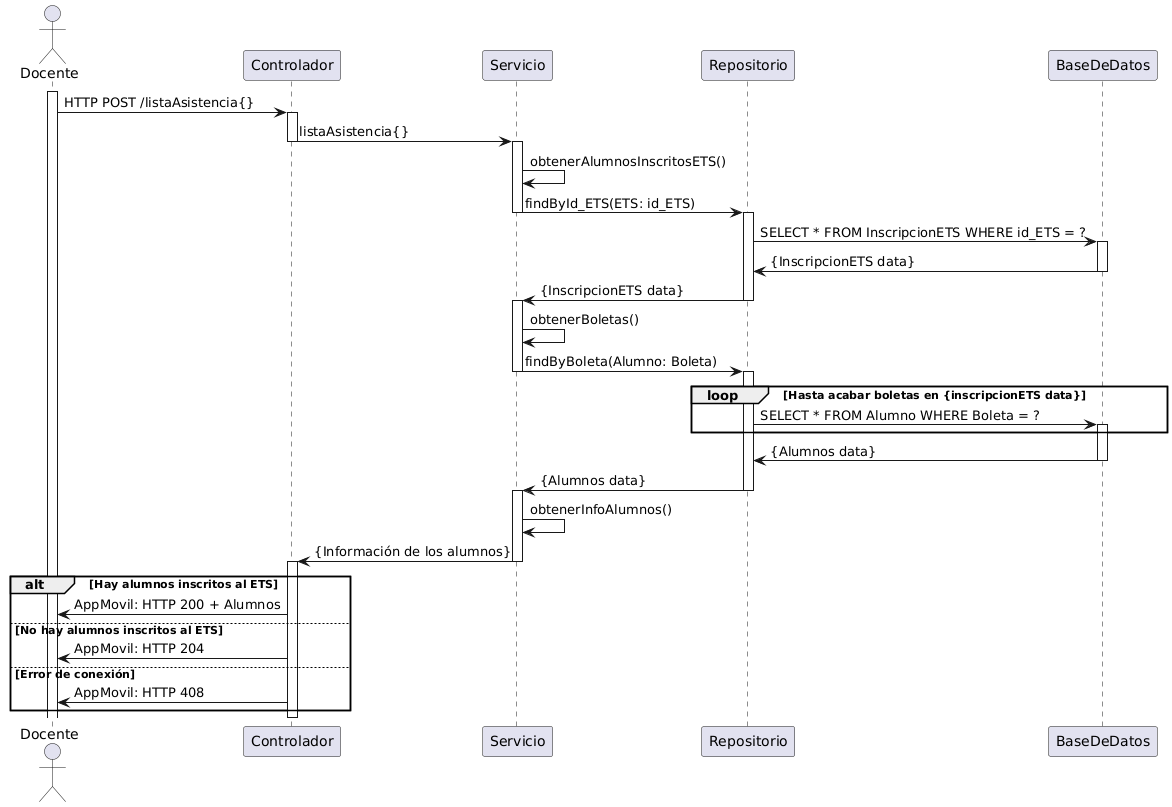
\includegraphics[width=1\textwidth]{Secuencia/CU-10.png}}
		\caption{Diagrama de secuencia del caso de uso número 10 (Consultar lista de asistencia de alumnos inscritos a los ETS).}
		\label{fig:Diagrama de secuencia CU-10}
	\end{center}
\end{figure}

En el diagrama de secuencia \ref{fig:Diagrama de secuencia CU-10} se describe el proceso planeado para el caso de uso \hyperlink{CU-10}{CU-10 Consultar lista de asistencia de alumnos inscritos a los ETS}, mostrando las interacciones que tendrá con la vista, el controlador, el servicio, el repositorio y la base de datos.

\newpage